\chapter{Технологический раздел}
\section{Обоснование выбора средств реализации базы данных и приложения}
Выбор PostgreSQL обусловлен его надежностью, производительностью и соответствием требованиям предметной области. Система предоставляет: полноценную поддержку ACID-транзакций для гарантии целостности данных, гибкую систему ограничений и триггеров для автоматизации бизнес-процессов, встроенную ролевую модель с детализированным управлением доступом, поддержку сложных типов данных (JSONB, ENUM), что упрощает хранение структурированной информации.

Для клиентской части выбор пал на $C\#$ в силу: строгой типизации и высокой производительности исполняемого кода, наличия проверенных инструментов интеграции с PostgreSQL (Npgsql), поддержки современных парадигм программирования и паттернов проектирования.

Данный технологический стек оптимально соответствует требованиям к безопасности, надежности и масштабируемости проектируемой системы учета.
\section{Реализация}
\subsection{Создание таблиц}
В листинге~\ref{lst:creation_of_tables} представлен код создания таблиц для базы данных Цветочный магазин.
\begin{lstlisting}[label=lst:creation_of_tables, caption=Создание таблиц базы данных, language=SQL]
	create table country(
	id int primary key,
	name text
	);
	
	create table nomenclature(
	id int primary key,
	name text,
	country_id int references country(id)
	);
	
	create type counterpart_role as enum ('поставщик', 'покупатель');
	create type legal_status_type as enum (
	'Физическое лицо',
	'Юридическое лицо',
	'Индивидуальный предприниматель'
	);
	
	create table counterpart(
	id int primary key,
	name text,
	type counterpart_role,
	legal_status legal_status_type,
	legal_address JSONB,
	contact_person text,
	phone varchar(20)
	);
	
	create type user_role as enum ('администратор', 'продавец', 'кладовщик');
	create table "user"(
	id int primary key,
	name text,
	type user_role
	);
	
	alter table "user" add column password varchar(255);
	
	create table batch_of_products(
	id_product_batch int,
	id_nomenclature int references nomenclature(id),
	production_date date,
	expiration_date date,
	cost_price decimal(12,2),  -- Себестоимость
	amount int,
	responsible int references "user"(id),
	suppliers int references counterpart(id),
	
	primary key (id_product_batch, id_nomenclature)
	);
	
	create table write_off(
	id int primary key,
	id_product_batch int,
	id_nomenclature int,
	amount int,
	responsible int references "user"(id),
	foreign key (id_product_batch, id_nomenclature) 
	references batch_of_products(id_product_batch, id_nomenclature)
	);
	
	create table price(
	id int primary key,
	id_nomenclature int REFERENCES nomenclature(id),
	selling_price decimal(12,2),  -- Цена продажи
	id_product_batch int,
	foreign key (id_product_batch, id_nomenclature) 
	references batch_of_products(id_product_batch, id_nomenclature)
	);
	
	create table storage_place(
	id int primary key,
	name text,
	address JSONB
	);
	
	
	CREATE TABLE product_in_stock(
	id int PRIMARY KEY,
	id_nomenclature int,
	id_product_batch int,
	amount int,
	storage_place int references storage_place(id),
	foreign key (id_product_batch, id_nomenclature) 
	references batch_of_products(id_product_batch, id_nomenclature)
	);
	
	create table "order"(
	id int primary key,
	reg_date date,
	counterpart int references counterpart(id),
	responsible int references "user"(id)
	);
	
	create table "order_product_in_stock"(
	id_order int references "order"(id),
	id_product int references product_in_stock(id),
	amount int,
	price int references price(id)
	);
	
	create type order_status_type as enum ('Новый', 'Подтверждён', 'Собран', 'Получен');
	
	create table sales(
	receipt_number int primary key,
	counterpart int references counterpart(id),
	order_id int references "order"(id),
	order_status order_status_type,
	final_price decimal(12,2)
	);
\end{lstlisting}
В листинге~\ref{lst:constraints} представлен код создания ограничений для таблиц базы данных Цветочный магазин.
\begin{lstlisting}[label=lst:constraints, caption=Создание ограничений для таблиц базы данных, language=SQL]
	-- Для таблицы country
	alter table country add constraint check_country_name_length check (length(name) > 0);
	
	-- Для таблицы nomenclature
	alter table nomenclature add constraint check_nomenclature_name_length check (length(name) > 0);
	alter table nomenclature add constraint check_country_reference check (country_id is not null);
	
	-- Для таблицы counterpart
	alter table counterpart add constraint check_counterpart_name_length check (length(name) > 0);
	alter table counterpart add constraint check_contact_person_length check (length(contact_person) > 0);
	alter table counterpart add constraint check_phone_format check (phone ~ '^\+?[0-9]{10,15}$');
	
	-- Для таблицы user
	alter table "user" add constraint check_user_name_length check (length(name) > 1);
	
	-- Для таблицы batch_of_products
	alter table batch_of_products add constraint check_production_date check (production_date <= current_date);
	alter table batch_of_products add constraint check_expiration_date check (expiration_date > production_date);
	alter table batch_of_products add constraint check_positive_cost_price check (cost_price > 0);
	alter table batch_of_products add constraint check_positive_amount check (amount > 0);
	
	-- Для таблицы write_off
	alter table write_off add constraint check_positive_write_off_amount check (amount >= 0);
	
	-- Для таблицы price
	alter table price add constaint check_positive_selling_price check (selling_price > 0);
	
	-- Для таблицы storage_place
	alter table storage_place add constraint check_storage_name_length check (length(name) > 0);
	
	-- Для таблицы product_in_stock
	alter table product_in_stock add constraint check_positive_stock_amount check (amount >= 0);
	
	-- Для таблицы order
	alter table "order_product_in_stock"
	add constraint fk_product_id foreign key (id_product) references product_in_stock;
	
	alter table "order_product_in_stock"
	add constraint fk_order_id foreign key (id_order) references "order";
	-- Для таблицы sales
	alter table sales ADD constraint check_positive_final_price check (final_price > 0);	
\end{lstlisting}
\subsection{Создание триггеров}
В листингах~\ref{lst:trigger1} и~\ref{lst:trigger2} представлены коды создания триггеров на обновление товара на складе при поступлении новой партии товара и на обновление товара на складе при покупке, соответственно.
\begin{lstlisting}[label=lst:trigger1, caption=Создание триггера на обновление товара на складе при поступлении новой партии товара, language=SQL]
create or replace function public.update_product_in_stock()
returns trigger
language plpgsql
as $function$
begin
	-- Проверяем, существует ли уже запись о данном товаре и партии на складе
	if exists (
	select 1 
		from product_in_stock 
		where id_nomenclature = new.id_nomenclature 
		and id_product_batch = new.id_product_batch
	) then
		-- Если запись существует, обновляем количество
		update product_in_stock
		set amount = amount + new.amount
		where id_nomenclature = new.id_nomenclature 
		and id_product_batch = new.id_product_batch;
	else
		-- Если записи нет, создаем новую
		insert into product_in_stock (id, id_nomenclature, id_product_batch, amount, storage_place)
		values (
			coalesce((select max(id) from product_in_stock), 0) + 1,
			new.id_nomenclature,
			new.id_product_batch,
			new.amount,
			(select id from storage_place order by random() limit 1) -- случайное место хранения
		);
		
		with avg_cost_by_year as (
			select 
				id_nomenclature,
				EXTRACT(YEAR FROM production_date) AS production_year,
				AVG(cost_price) * 1.55 AS calculated_price
			from 
				batch_of_products
			group by
				id_nomenclature, 
				extract(year from production_date)
		)
		insert into price (id, id_nomenclature, selling_price, id_product_batch)
		select 
			row_number() over () + coalesce((select max(id) from price), 0),
			bop.id_nomenclature,
			ac.calculated_price,
			bop.id_product_batch
		from 
			batch_of_products bop 
		join 
			avg_cost_by_year ac on bop.id_nomenclature = ac.id_nomenclature 
			and extract(year from bop.production_date) = ac.production_year
		where bop.id_nomenclature = new.id_nomenclature and bop.id_product_batch = new.id_product_batch;
	end if;
	
	return new;
end;
$function$
;
\end{lstlisting}

\begin{lstlisting}[label=lst:trigger2, caption=Создание триггера на обновление товара на складе при покупке, language=SQL]
create or replace function public.update_stock_on_order_product_insert()
returns trigger
language plpgsql
as $function$
declare
	batch_rec record;
	remaining_amount numeric := new.amount;
	nomencl_id int;
	price_rec record;
begin
	-- Получаем id_nomenclature из связанной записи product_in_stock
	select id_nomenclature into nomencl_id 
	from product_in_stock 
	where id = new.id_product;
	
	-- Проверяем доступное количество с учетом срока годности
	while remaining_amount > 0 loop
		-- Ищем подходящую партию с неистекшим сроком годности
		select pis.id, pis.amount, p.id as price_id, bop.expiration_date
		into batch_rec
		from product_in_stock pis
		join batch_of_products bop on pis.id_product_batch = bop.id_product_batch
		and pis.id_nomenclature = bop.id_nomenclature
		join price p on p.id_nomenclature = bop.id_nomenclature
		and p.id_product_batch = bop.id_product_batch
		where pis.id_nomenclature = nomencl_id
		and pis.amount > 0
		and bop.expiration_date > current_date
		order by bop.expiration_date asc, pis.amount desc
		limit 1
		for update of pis;
		
		if not found then
			raise exception 'Недостаточно товара на складе с неистекшим сроком годности. ID товара: %, запрошено: %, осталось: %', 
			new.id_product, 
			new.amount,
			new.amount - remaining_amount;
		end if;
		
		-- Определяем сколько можем списать с этой партии
		declare
			to_reduce numeric := least(batch_rec.amount, remaining_amount);
		begin
			-- Списание
			update product_in_stock
			set amount = amount - to_reduce
			where id = batch_rec.id;
			
			-- Сохраняем цену в заказе
			if remaining_amount = new.amount then
				new.price := batch_rec.price_id;
			end if;
			
			remaining_amount := remaining_amount - to_reduce;
		end;
	end loop;
	
	return new;
end;
$function$
;
\end{lstlisting}

\subsection{Создание ролей}
В листинге~\ref{lst:roles} представлен код создания ролей для базы данных Цветочный магазин.
\begin{lstlisting}[label=lst:roles, caption=Создание ролей для базы данных, language=SQL]
-- Создаем роли
create role flower_admin with login password 'admin_password';
create role flower_seller with login password 'seller_password';
create role flower_storekeeper with login password 'storekeeper_password';

-- Комментарии к ролям
comment on role flower_admin is 'Администратор цветочного магазина (полные права)';
comment on role flower_seller is 'Продавец (просмотр товаров, оформление заказов)';
comment on role flower_storekeeper is 'Кладовщик (просмотр товаров, загрузка партий)';

-- Права для кладовщика
grant select on nomenclature, price, product_in_stock, batch_of_products, country to flower_storekeeper;
grant insert on price to flower_storekeeper;
grant insert on batch_of_products to flower_storekeeper;
grant select, insert on product_in_stock to flower_storekeeper;
grant select on storage_place to flower_storekeeper;
-- Права на последовательности (если используются автоинкрементные ID)
grant usage, select on ALL SEQUENCES IN SCHEMA public to flower_storekeeper;
grant usage on schema public to flower_storekeeper;
grant execute on function update_product_in_stock() to flower_storekeeper;

-- Права для продавца
grant flower_storekeeper to flower_seller;
grant insert, select on "order", order_product_in_stock, sales to flower_seller;
grant update (amount) on product_in_stock to flower_seller;
grant select on "user" to flower_seller;

grant select on product_in_stock to flower_seller;
grant select on batch_of_products to flower_seller;
grant select on price to flower_seller;
grant execute on function update_stock_on_order_product_insert() to flower_seller;

-- Права для администратора
grant flower_storekeeper to flower_admin;
grant flower_seller to flower_admin;

\end{lstlisting}
\section{Тестирование}
В таблице~\ref{tab:tests} приведены тесты для проверки корректности работы триггеров. Для этого были написаны интеграционные тесты.
\begin{table}[h]
	\centering
	\caption{Тестирование корректности работы триггеров и ограничений}
	\label{tab:tests}
	\begin{tabular}{|p{3cm}|p{3cm}|p{4cm}|p{4cm}|}
		\hline
		\textbf{Название} & \textbf{Входные данные} & \textbf{Ожидаемый результат} & \textbf{Фактический результат} \\
		\hline
		Триггер на обновление товара на складе при поступлении новой партии товара. & Корректные данные. & Добавление соответствующих строк в таблицы $batch~of~products$, $product~in~stock$ и $price$. & Нужные строки были добавлены.  \\
		\hline
		Триггер на обновление товара на складе при поступлении новой партии товара. & Данные с повторяющемся номером партии & Вызов исключения. & Ошибка при загрузке партии: 23505: повторяющееся значение ключа нарушает ограничение уникальности "batch of products pkey"  \\
		\hline
		Триггер на обновление товара на складе при покупке. & Корректные данные. & Добавление соответствующих строк в таблицы $order$, $sales$ и изменение количества соответствующего товара в таблице $product~in~stock$. & Нужные строки были добавлены и количество в наличие было изменено.  \\
		\hline
		Триггер на обновление товара на складе при покупке. & Попытка купить больше чем есть в наличие. & Вызов исключения. & Исключение 'Недостаточно товара на складе с неистекшим сроком годности.' \\
		\hline
	\end{tabular}
\end{table}

Также были написаны модульные тесты для программы управления базой данных.
Результат тестирования представлен на изображении~\ref{fig:tests}
\begin{figure}
	\centering
	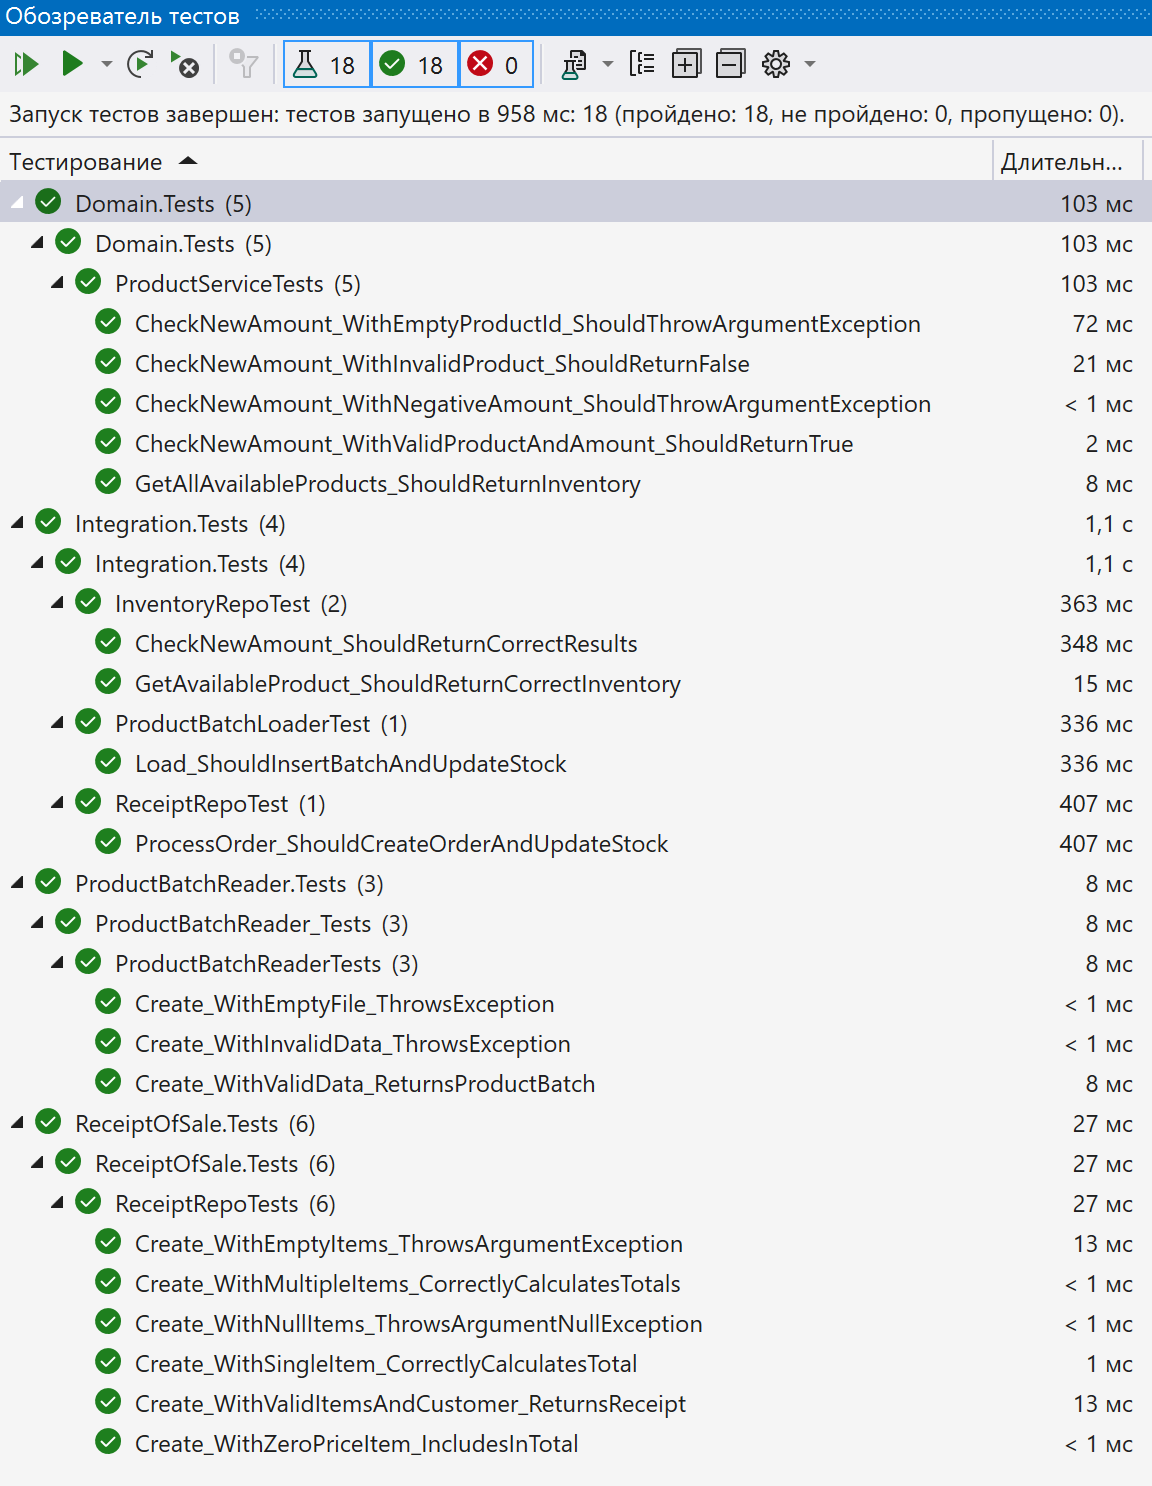
\includegraphics[width=1\linewidth]{pictures/tests}
	\caption{Результат модульного и интеграционного тестирования}
	\label{fig:tests}
\end{figure}
\clearpage
\section{Пример работы программы}
В листинге~\ref{lst:prog_buy} представлен пример работы программы для сценария совершения покупки. Многоточием заменены постоянно повторяющийся вывод меню.
\begin{lstlisting}[label=lst:prog_buy, caption=Совершение покупки, language=SQL]
	Введите логин (Ваш ID): 1
	Введите пароль: pass1
	Вы вошли как администратор.
	=== ГЛАВНОЕ МЕНЮ ===
	1. Сделать заказ
	2. Загрузка информации о новой партии
	0. Выход
	Выберите пункт меню: 1
	=== Сделать заказ ===
	1. Показать доступные товары
	2. Добавить товар в корзину
	3. Изменить количество товара в корзине
	4. Удалить товар из корзины
	5. Показать содержание корзины
	6. Заказать
	0. Назад (если вернуться, содержание корзины обнулится)
	Выберите пункт меню: 1
	Товар: 1 Телопея, United Kingdom, количество: 32, цена: 3725,24
	Товар: 4 Сетария, Cape Verde, количество: 2, цена: 5260,35
	Товар: 5 Амбрелла, Bolivia, количество: 55, цена: 3703,16
	Товар: 9 Антуриум, Botswana, количество: 27, цена: 4181,22
	Товар: 11 Ваза керамическая белая 25см, Zimbabwe, количество: 23, цена: 6872,71
	Товар: 13 Книфофия, Philippines, количество: 45, цена: 3888,72
	Товар: 15 Сетка декоративная медовая 45смx100м, Namibia, количество: 60, цена: 4255,04
	Товар: 19 Лента репсовая Пудра 100м, Uganda, количество: 11, цена: 4667,08
	Товар: 21 Эрика, Tanzania, количество: 2, цена: 5698,18
	Товар: 23 Пион, Turkmenistan, количество: 53, цена: 4522,5
	Товар: 36 Пихта, Andorra, количество: 13, цена: 3515,79
	Товар: 44 Вибурнум, Monaco, количество: 4, цена: 3889,92
	Товар: 45 Пион, Iraq, количество: 9, цена: 5187,55
	Товар: 51 Кипарисовик, United States of America, количество: 47, цена: 4526,53
	Товар: 56 Тилландсия, Grenada, количество: 7, цена: 3207,71
	Товар: 61 Лента атласная красная 100м, Mexico, количество: 3, цена: 3909,84
	Товар: 64 Лента рафия окрашенная (10 цветов) 100м, Dominican Republic, количество: 1, цена: 5139,66
	Товар: 66 Подставка для вазы 30см, Haiti, количество: 84, цена: 2917,62
	Товар: 67 Лента атласная золотая 100м, The Gambia, количество: 12, цена: 3458,98
	Товар: 70 Астильба, Democratic Republic of Congo, количество: 6, цена: 3005,13
	______________________________________________________________________
	Продолжить вывод доступных товаров? (0 - остановиться, 1 - продолжить): 0
	=== Сделать заказ ===
	...
	Выберите пункт меню: 2
	Введите id товара для добавления в корзину: 5
	Введите количество товара для добавления в корзину: 10
	Товар добавлен в корзину.
	=== Сделать заказ ===
	...
	Выберите пункт меню: 2
	Введите id товара для добавления в корзину: 66
	Введите количество товара для добавления в корзину: 14
	Товар добавлен в корзину.
	=== Сделать заказ ===
	...
	Выберите пункт меню: 5
	Корзина:
	5 Амбрелла, Bolivia, количество: 10, цена за шт.: 3703,16
	66 Подставка для вазы 30см, Haiti, количество: 14, цена за шт.: 2917,62
	=== Сделать заказ ===
	...
	Выберите пункт меню: 6
	Заказ оформлен. Номер чека 5024
\end{lstlisting}
В листинге~\ref{lst:prog_load} представлен пример работы программы для сценария загрузки информации о новой партии. 
\begin{lstlisting}[label=lst:prog_load, caption=Загрузка информации о новой партии товара, language=SQL]
	Введите логин (Ваш ID): 1
	Введите пароль: pass1
	Вы вошли как администратор.
	=== ГЛАВНОЕ МЕНЮ ===
	1. Сделать заказ
	2. Загрузка информации о новой партии
	0. Выход
	Выберите пункт меню: 2
	=== Загрузка информации о новой партии ===
	Введите путь к файлу с данными о партии:
	"D:\bmstu\Курсовая по БД\software_design\ProjectForCourseWorkForDB\FlowerShop\batch4.txt"
	Needs to be loaded
	  Номенклатура Даты (произв./годен)      Кол-во Цена           Срок годности   
	  854          30.05.2025 / 30.05.2026   51     1404,50 руб.   363 дней        
	  626          30.05.2025 / 28.08.2025   39     4590,14 руб.   88 дней        
	  646          30.05.2025 / 28.08.2025   69     3887,61 руб.   88 дней        
	  383          30.05.2025 / 13.06.2025   60     3958,11 руб.   12 дней        
	  705          30.05.2025 / 13.06.2025   8      1054,00 руб.   12 дней        
	  205          30.05.2025 / 29.06.2025   66     2568,34 руб.   28 дней        
	  55           30.05.2025 / 26.11.2025   71     1962,61 руб.   178 дней        
	  340          30.05.2025 / 29.07.2025   16     1384,28 руб.   58 дней        
	  109          30.05.2025 / 30.05.2026   71     1115,37 руб.   363 дней        
	  901          30.05.2025 / 06.06.2025   63     4529,26 руб.   5 дней        
	  98           30.05.2025 / 29.07.2025   8      3565,52 руб.   58 дней        
	  311          30.05.2025 / 29.07.2025   12     1847,95 руб.   58 дней        
	  425          30.05.2025 / 30.05.2026   54     4314,36 руб.   363 дней        
	  33           30.05.2025 / 26.11.2025   48     2973,71 руб.   178 дней        

	Загрузка прошла успешно!
	=== ГЛАВНОЕ МЕНЮ ===
	1. Сделать заказ
	2. Загрузка информации о новой партии
	0. Выход
	Выберите пункт меню: 1
	=== Сделать заказ ===
	1. Показать доступные товары
	2. Добавить товар в корзину
	3. Изменить количество товара в корзине
	4. Удалить товар из корзины
	5. Показать содержание корзины
	6. Заказать
	0. Назад (если вернуться, содержание корзины обнулится)
	Выберите пункт меню: 1
	Товар: 1 Телопея, United Kingdom, количество: 32, цена: 3725,24
	Товар: 4 Сетария, Cape Verde, количество: 2, цена: 5260,35
	Товар: 5 Амбрелла, Bolivia, количество: 45, цена: 3703,16
	Товар: 9 Антуриум, Botswana, количество: 27, цена: 4181,22
	Товар: 11 Ваза керамическая белая 25см, Zimbabwe, количество: 23, цена: 6872,71
	Товар: 13 Книфофия, Philippines, количество: 45, цена: 3888,72
	Товар: 15 Сетка декоративная медовая 45смx100м, Namibia, количество: 60, цена: 4255,04
	Товар: 19 Лента репсовая Пудра 100м, Uganda, количество: 11, цена: 4667,08
	Товар: 21 Эрика, Tanzania, количество: 2, цена: 5698,18
	Товар: 23 Пион, Turkmenistan, количество: 53, цена: 4522,5
	Товар: 33 Молюцелла, Uganda, количество: 48, цена: 3963,05
	Товар: 36 Пихта, Andorra, количество: 13, цена: 3515,79
	Товар: 44 Вибурнум, Monaco, количество: 4, цена: 3889,92
	Товар: 45 Пион, Iraq, количество: 9, цена: 5187,55
	Товар: 51 Кипарисовик, United States of America, количество: 47, цена: 4526,53
	Товар: 55 Мускари, Lebanon, количество: 71, цена: 3631,19
	Товар: 56 Тилландсия, Grenada, количество: 7, цена: 3207,71
	Товар: 61 Лента атласная красная 100м, Mexico, количество: 3, цена: 3909,84
	Товар: 64 Лента рафия окрашенная (10 цветов) 100м, Dominican Republic, количество: 1, цена: 5139,66
	Товар: 66 Подставка для вазы 30см, Haiti, количество: 70, цена: 2917,62
\end{lstlisting}
\section*{Вывод}
\addcontentsline{toc}{section}{Вывод}
В рамках технологического раздела была успешно реализована база данных цветочного магазина, включающая все необходимые таблицы, ограничения целостности и триггеры для автоматизации бизнес-процессов. Разработанное приложение на $C\#$ обеспечило удобный интерфейс для взаимодействия с системой. Проведенные интеграционные и модульные тесты подтвердили корректность работы всех компонентов.